% !TEX TS-program = pdflatexmk
\documentclass[review]{elsarticle}
\usepackage{graphicx}
\usepackage{epstopdf}
\usepackage{float}
\usepackage[numbers]{natbib}
\usepackage{lineno}
\usepackage{numcompress}
\usepackage{amssymb}
\usepackage{subcaption}
\usepackage{tabularx}
\usepackage{hyperref}
\usepackage{siunitx}
\usepackage{booktabs}
\usepackage{scrextend}

\modulolinenumbers[5]
\graphicspath{{figs/}}

\DeclareGraphicsRule{.tif}{png}{.png}{`convert #1 `dirname #1`/`basename #1 .tif`.png}

\def\vm{VaxiMap}
\newcommand{\coo}{\ensuremath{\mathrm{CO_2}}}

\graphicspath{{figs/}{../analysis}{../survey}}

\begin{document}

\begin{frontmatter}

\title{\vm{}{}: optimal delivery of vaccinations for housebound patients}


\address[IBME]{Institute of Biomedical Engineering, Department of Engineering Science, University of Oxford}
\cortext[mycorrespondingauthor]{Corresponding author}

\address[Sqpt]{Squarepoint Capital LLP, London}
\address[Vod]{Vodafone Group PLC, London}

\author[IBME]{Thomas Kirk\corref{mycorrespondingauthor}}
\ead{tomfrankkirk@gmail.com}

\author[Sqpt]{Adam Barker}
\author[Vod]{Armen Bodossian}
\author[IBME]{Robert Staruch}

\begin{abstract}
\paragraph{Background} During the UK's Covid-19 vaccination campaign, responsibility for vaccinating housebound patients has rested with individual GP surgeries, posing them a difficult logistical challenge (the travelling salesman problem). In response to demand from GPs, and a lack of solutions tailored specifically to vaccination, a tool for the optimisation of vaccine delivery to these patients, entitled \vm{}, was made available free-of-charge in January 2021. 

\paragraph{Methods} \vm{} generates optimal routes subject to the constraint that the number of patients per route should be fixed. This ensures that a known quantity of vaccine can be set aside for each route and minimises wastage. The user need only upload an Excel spreadsheet of patient postcodes to be visited; a divide-and-conquer approach of iterative $k$-means clustering followed by within-cluster route optimisation is used. 

\paragraph{Findings} We find substantial savings in the time taken to plan vaccinations, and smaller savings in the time taken to visit housebound patients. We estimate savings to date of 4394 hours of practitioner time, equivalent to 109 weeks at 40 hours/week or approximately £85k at typical practitioner salaries. 

\paragraph{Interpretation} The adoption of \vm{} yielded both time and cost savings for GP surgeries and accelerated the UK's Covid-19 vaccination campaign at a critical moment. 

\paragraph{Funding} Financial support for \vm{} was provided by Magdalen College, Oxford, Oxford University Innovation, and JHubMed, part of UK Strategic Command. These parties were not involved in the preparation of this manuscript. 

\begin{keyword}
vaccination \sep covid-19 \sep housebound \sep optimisation \sep travelling salesman
\end{keyword}

\end{abstract}

\end{frontmatter}

\linenumbers

\section{Research in context} 

\subsection{Evidence before this study} A search on Google Scholar for \textit{optimal housebound patient home visit travelling salesman} shows that multiple authors have investigated variations on the basic travelling salesman problem in the context of healthcare. Analyses using both novel and existing solutions show that important time savings can be obtained using route optimisation. A search for \textit{human performance travelling salesman} shows that humans can produce viable solutions to the problem, though the time taken for this is generally not reported precisely. Importantly, previous work does not address problems that start with a non-visual representation of the locations to be visited, which is an import aspect of the problem addressed here. No date criterion was used to exclude studies from the literature search. 

\subsection{Added value of this study} At the time this work was undertaken (January - March 2021), existing solutions to the travelling salesman problem were not being widely used by GP surgeries to support vaccination. Hence, in light of large demand and the urgency of the situation, a domain-specific solution was built. Our results show that this solution yielded time and cost savings, accelerating the UK's Covid-19 vaccination campaign. 

\subsection{Implications of all the available evidence} Route optimisation is a simple and widely available technology. In agreement with the existing body of work, our results imply that route optimisation for the delivery of services besides vaccination to housebound patients would yield further savings. 

\section{Background}
\label{sec:background}

In early 2021 a global campaign to vaccinate against SARS-COV2 was launched. In the UK, the Joint Committee on Vaccination and Immunisation (JCVI) stipulated that patients should be vaccinated in descending age and risk order. Under the nine risk categories identified by the JCVI, housebound patients were allocated into the higher priority groups for early vaccination. 

There are estimated to be on the order of half a million housebound patients in the UK\footnote{Numerous freedom of information requests to NHS England, Public Health England and the JCVI have not yielded a precise figure. Correspondence with a member of the Health Informatics Group at the Royal College of General Practitioners suggests a lower bound of 250,000.}. Responsibility for vaccinating these patients has lain with  general practitioner (GP) surgeries as they cannot present at a mass vaccination centre. In order for the wider vaccination campaign to proceed on schedule, it was therefore of vital importance that GPs could quickly and efficiently deliver vaccinations to these patients. Given their high risk profile, timely vaccination would also reduce the burden on other parts of the health system. 

The central problem in optimising the vaccination of housebound patients is determining the fastest order in which to visit the individuals. This is an example of the travelling salesman problem (TSP), which has been extensively studied in the domain of computer science. Notwithstanding numerous solutions to the problem \cite{Laporte1990}, some of which have been applied in a medical context \cite{Shao2012}, vaccination imposes an extra constraint. Because there are a fixed number of doses in a vial, it is preferable sort patients into groups of this same number. This ensures that exactly one vial (or integer multiple thereof) of vaccine will be required per group of visited patients. Separately, due to the cold-storage requirements of the vaccines themselves, visiting patients in in the fastest order minimises the time that vials spend outside of the cold chain. Taken together, these two factors reduce vaccine wastage, especially important given the limited supplies available during the early stages of the campaign. 

Though commercial solutions for route planning exist, these were not widely adopted by GPs for use in the vaccination campaign, possibly because they do not allow for constraints on group size. In response to numerous requests for help from GPs and practice managers on social media, it was therefore decided to build a domain-specific solution entitled \vm{} (\hyperlink{https://www.vaximap.org}{www.vaximap.org}) in January 2021. The service is a free-to-use website that requires only an excel spreadsheet of patient postcodes to function. The patients are then sorted into groups of fixed size based on proximity to each other, the fastest route within each found, and directions and estimated travel times returned to the user (an example is shown in figure \ref{demo}). Within a month of starting up, over 100,000 vaccine deliveries had been planned on the site; as of December 2021 the number stood at 365,000. This level of usage was reached purely via word of mouth amongst the GP community; at no point did the NHS or other central authority encourage uptake. 

\begin{figure}[htbp]
\centering
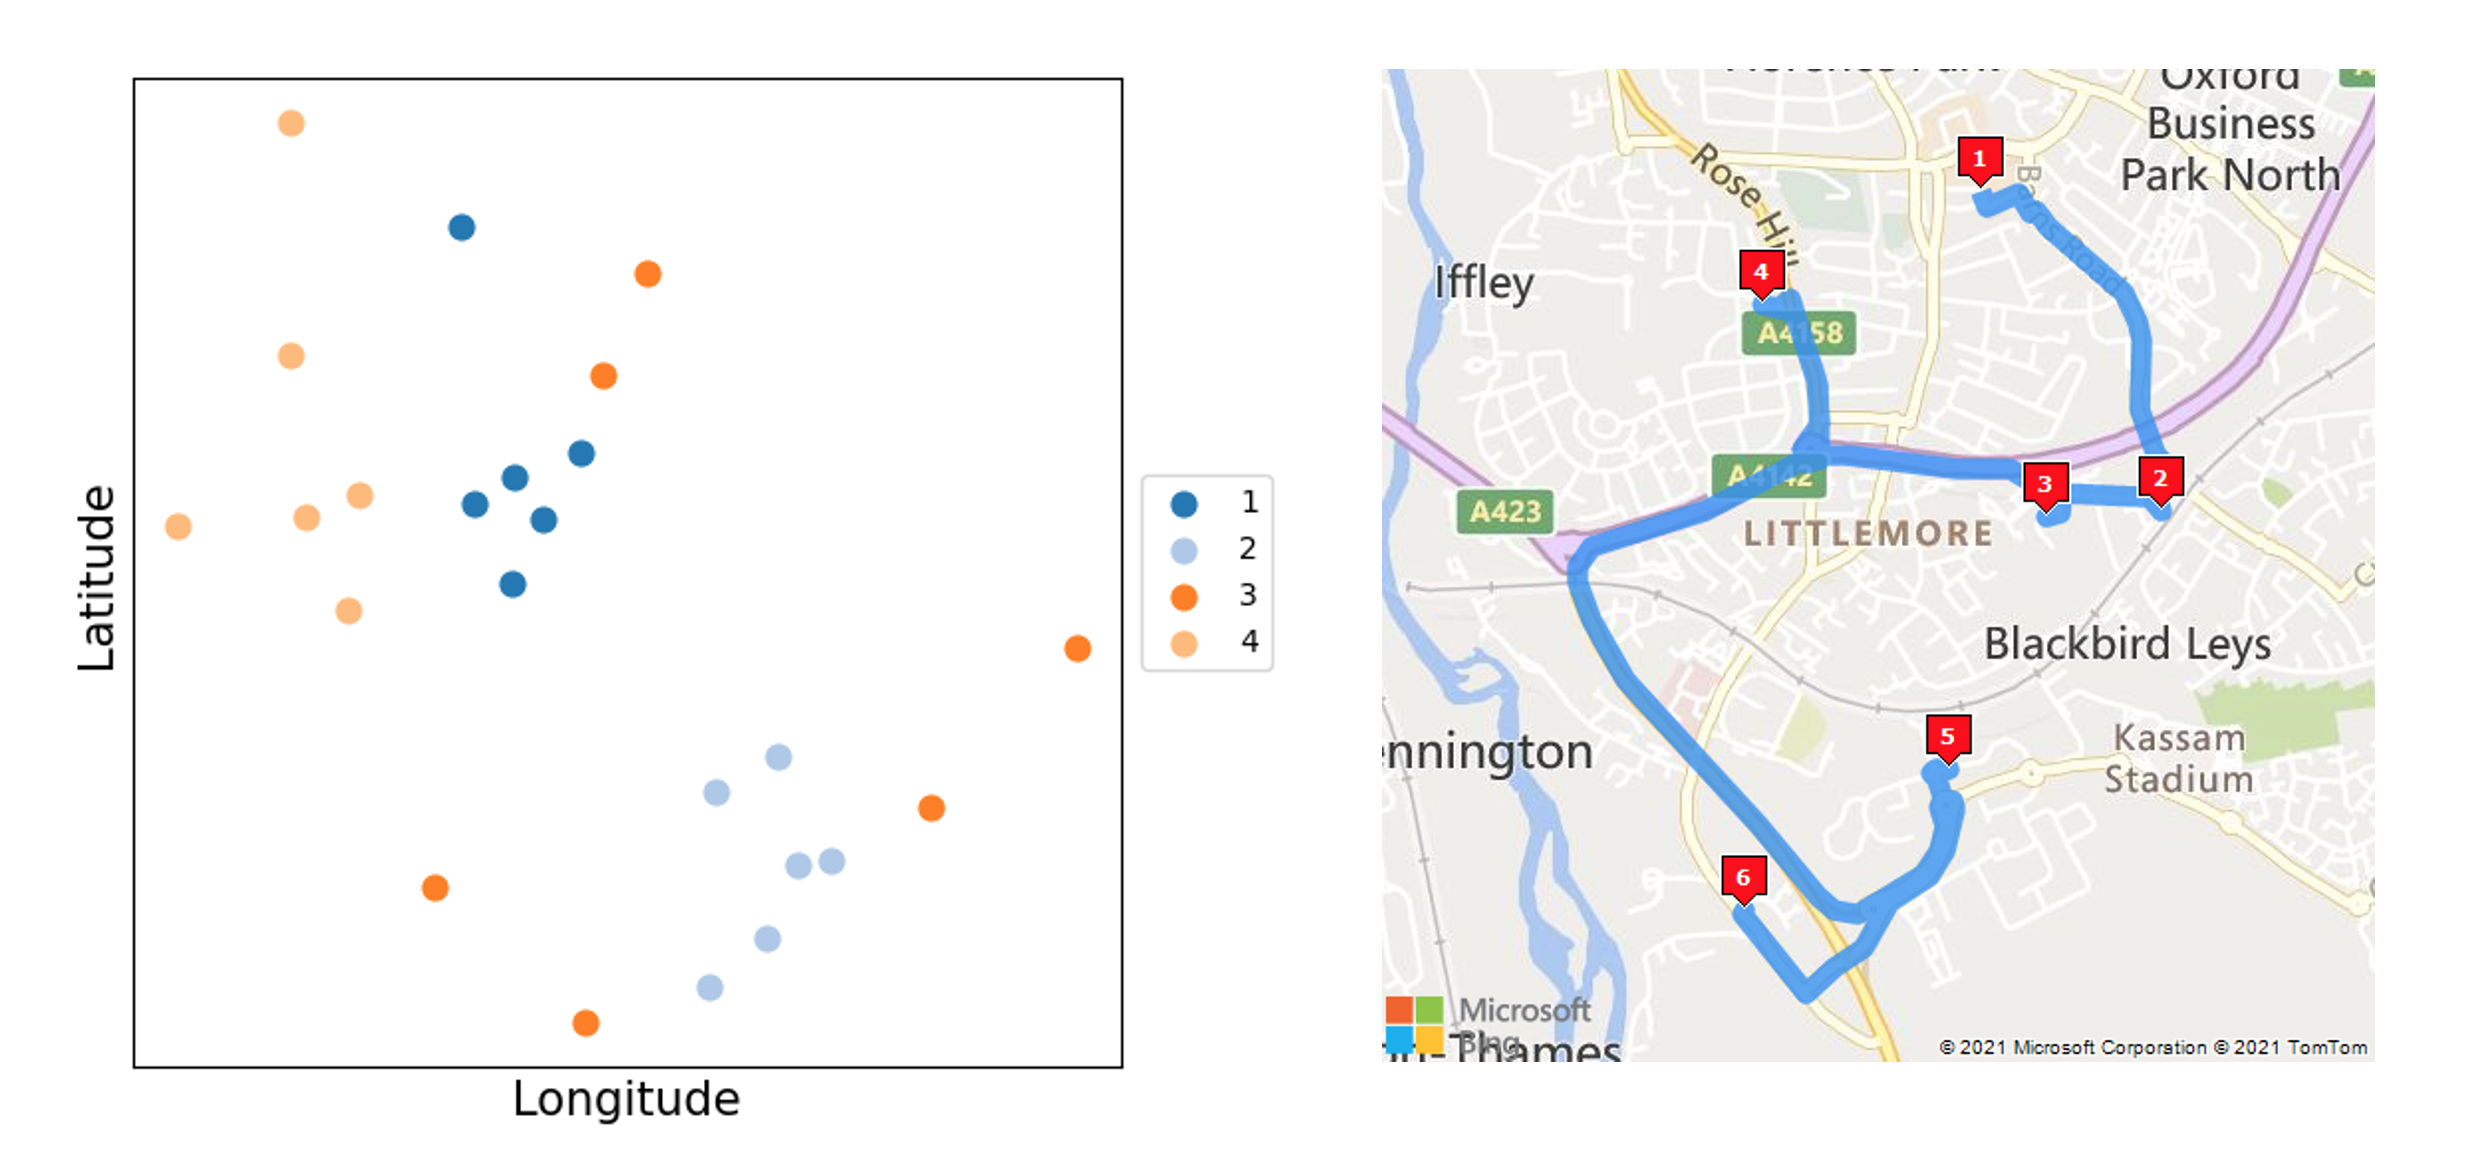
\includegraphics[width=\textwidth]{demo.png}
\caption{Example output produced by \vm{}. Left: 24 patients have been sorted into 4 clusters, the spatial distribution of which is shown here. Right: the optimal driving route for visiting the patients in cluster no. 2 (light blue).}
\label{demo}
\end{figure}

The purpose of this paper is to explain how the service functions and to estimate the beneficial impact it has had (via time savings in vaccine delivery). The data from which these estimates are derived (freely accessible in the public domain at [DOI link will be inserted after review]), analysis, and conclusions we present are of interest to public health officials involved in the delivery of services to housebound patients, be they vaccination-related or otherwise. 

\section{Methods \& Materials}
\subsection{Implementation}

The problem is defined as finding the shortest routes to visit a set of $N$ patients, whilst ensuring any individual practitioner visits no more than $D$ patients at a time. It is assumed, but not required, that $D$ is set as the number of vaccine doses in a vial (for example, nine for Oxford-AstraZeneca); any number between 3 and 25 can be used. It follows that the $N$ patients must be sorted into $G = \mathrm{ceiling}(N / D)$ groups (rounded up in the case that $D$ does not divide perfectly into $N$, in which case \textit{exactly} one group will have size less than $D$)\footnote{This is an important extra constraint added at the request of a GP, which ensures at most one vial of vaccine will be incompletely consumed.}. 

Patient postcodes uploaded by the user are transformed into latitude and longitude coordinates on the $x,y$ plane via the use of Microsoft Bing's \textit{geocoding} service. Next, the patients are grouped so that they are proximal in space, a simple heuristic to minimise the travel time \textit{within} each group. Iterative $k$-means clustering is used to group the patients subject to the constraint on group size $D$ (which standard $k$-means cannot do) \cite{macqueen1967some, davidson2005clustering}. Qualitatively, this approach assigns those patients that are far away from all others first, as these must be placed into the `correct' group, whereas those that are close the centre of the distribution can be assigned to any group with little consequence. The clustering process is illustrated in figure \ref{clustering}. 

\begin{figure}[htbp]
\centering
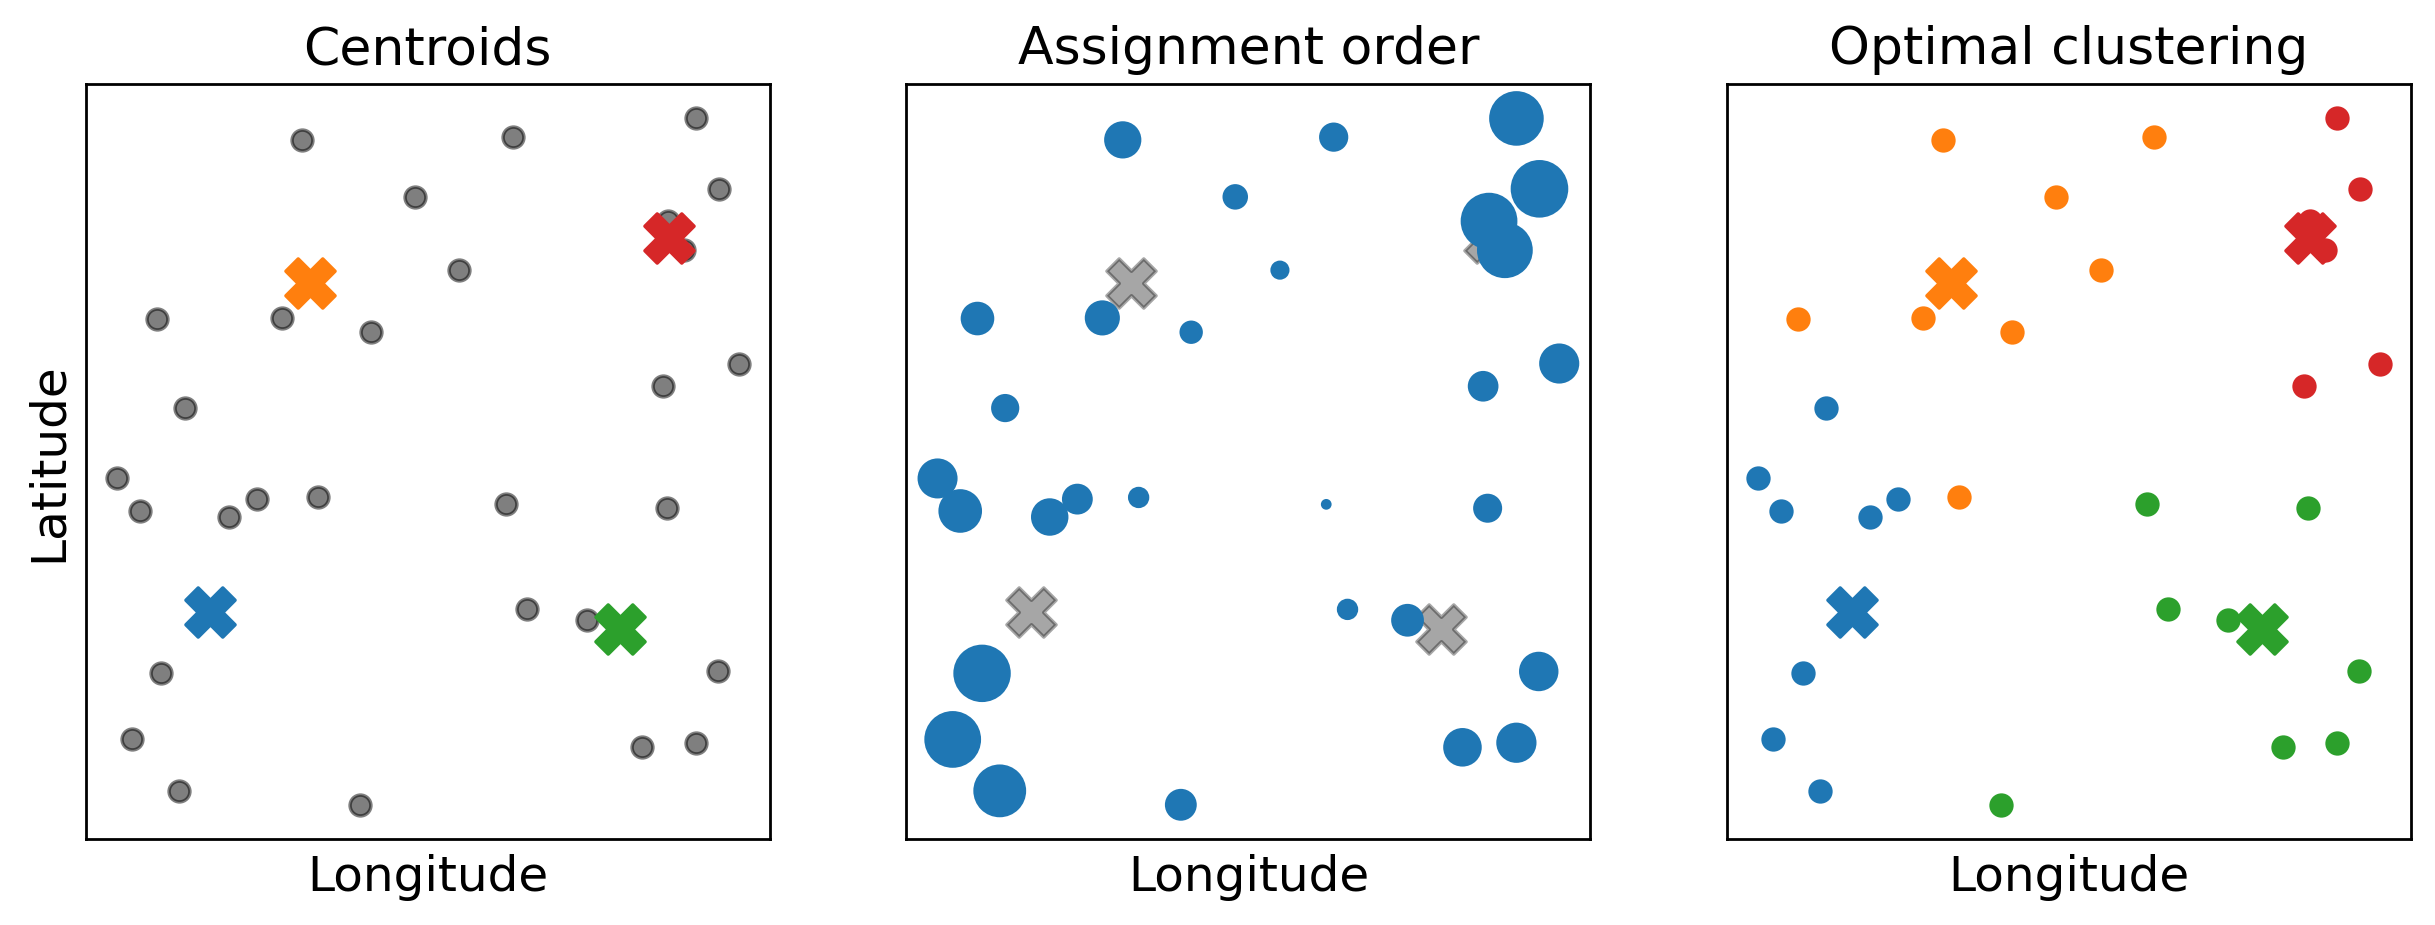
\includegraphics[width=\textwidth]{clustering_demo.png}
\caption{Example clustering of 30 patients into groups of eight. Left: initialisation of four cluster centroids (denoted with crosses). Centre: order of patient assignment, where larger circles indicate priority. Patients in the centre of the distribution could be assigned to any cluster with low cost, so are dealt with last. Right: the optimal clustering of patients after assignment. The red cluster has six patients due to imperfect number division, whereas all other clusters are fully-sized.}
\label{clustering}
\end{figure}

After cluster assignment, the final step is to determine the optimal order in which to visit the patients of each group. This is achieved via Microsoft Bing’s mapping API, making use of the \textit{optimise waypoints} facility (which imposes a limit of 25 patients per group) \cite{msbing}. Optionally, the user can specify a fixed start and end point for their routes (for example, the address of their GP surgery); each route will then be a round-trip from that location. The user is returned the patient groups, the optimal driving or walking directions within each group, and travel time estimates for each group. 

\subsection{Dataset}

Since the launch of the \vm{} service in January, a database of generated routes has been accumulated. From each user \textit{request} (corresponding to a single upload of patient postcodes and the routes that result), the following data are retained: time and date; number of patients; requested cluster size; relative distances between patients (not absolute locations); and transport mode. For approximately a third of requests, a histogram of patient postcode districts\footnote{Typical postal districts have in excess of 10,000 patients \cite{OfficeforNationalStatistics}, so this information is geographically non-precise.} was also retained (postal district is the first part of a postcode, for example OX1). As of December 2021, the dataset comprises 9,500 requests for 365,000 patients and has been released into the public domain alongside this work [DOI link will be inserted after review]. Postal district information is available for 3,100 of the requests. 

\subsection{Analysis methods}

The objective of analysis was to estimate the time savings yielded by \vm{} and identify high-level trends in how the service has been used. The savings arise in two ways: firstly, when \textit{planning} a route to visit patients; and secondly when \textit{following} an optimal route instead of a sub-optimal one. The following analysis was performed. 

\paragraph{Repeat detection}
In the course of development, it was noted that users sometimes uploaded the same set of patients multiple times in quick succession, with slightly different parameters. It is suspected that such behaviour reflects a learning process on the part of users who were familiarising themselves with the site. For certain analyses, such repeat requests (defined as request created within 21 days of a previous identical request) were removed. It was not desired to strip out repeats separated by more than 21 days as these could represent genuine repeat uses, though they may not correspond to repeat vaccinations if separated by just a few weeks. 

\paragraph{Summary metrics}
Summary metrics of the dataset were explored by drawing histograms of the number of patients uploaded per request, the number of clusters the request was split into, and the number of patients per cluster. The time-series nature of the data was explored by plotting the number of user requests per day, and the total number of patients across all requests per day. Finally, the geographic distribution of the data was exploited by plotting cumulative number of patients across all requests in each UK postal district on the postcode subset data. These analyses were performed on the dataset with repeats. 

\paragraph{Route planning}
The time taken for humans to plan solutions for the TSP is remarkably quick and scales linearly with the number of locations to be visited \cite{Macgregor1996, Dry2006, MacGregor2011}. The problem solved by \vm{} is subtly different to the conventional TSP investigated in the literature because users are starting with a text-based list of addresses (\textit{i.e}, from an EMIS database) as opposed to a visual representation. This difference is important in light of the consensus view that ``humans require a visual representation of the problem'' in order to solve the problem effectively \cite{MacGregor2011}. The time taken to plan routes in the absence of \vm{} can therefore be split into two components: a \textit{lookup time} to generate a spatial representation of the problem, and a \textit{routing time} to actually plan the routes using said representation. A survey that investigated both of these components separately was conducted across 19 volunteers (6 female, mean age 45 years, further information given in the supplementary material). Linear regressions across their responses yielded the following estimates for the time taken to perform these tasks manually: 37·0 seconds for lookup time, and 4·7 seconds for planning time, where both quantities are given per patient (uncertainties are given in the supplementary material). These coefficients were then multiplied across the entire dataset, including repeats, to obtain estimates of the time saved in planning. Repeats were included in this analysis as it was assumed users had reasonable cause for them (for example, experimenting with different cluster sizes and observing the differing travel times that result before making a decision). 

\paragraph{Route following}
The quality of human solutions to the TSP has been investigated extensively \cite{Vickers2001, MacGregor1999a, MacGregor2011, Macgregor1996}. These are often remarkably close to optimal for small problems and scale well  for larger problems ($n > $ 50 locations). The empirical model of performance given in figure 2b of Dry's review \cite{Dry2006}, reproduced below in figure \ref{dry_model}, was used in this work to approximate the extra distance penalty $p(n)$ of human solutions compared to \vm{}'s solution. The penalty is very small for problems with $n \leq$ 25 patients. For each user request in the non-repeated dataset, the total (closed) length of the \vm{} generated routes $L_{vm}$ was calculated and multiplied by a scaling factor $(1 + p(n))$ drawn from figure \ref{dry_model} to obtain an approximation for the length of the human solution to the same problem. Finally, in order to reflect the fact that real-world distances are not straight lines, though the dataset records them as such, a detour index $d$ (ratio of real world distance to straight line distance) of 1·4 was used in this work \cite{Cole1968}. Thus, the total length of a human solution was calculated as $L_{h} = L_{vm} \cdot (1 + p(n)) \cdot d$. In order to convert distance savings into time savings, a mean driving speed of 50 km/h or 30 mph was assumed \cite{Balendra2020}. Repeats were not included in this estimate as it was assumed to be unlikely that the journeys themselves were undertaken (though a user may have planned the same route twice in a week, they are unlikely to have actually undertaken it twice).  

\begin{figure}[H]
\centering
\includegraphics[width=0.7\textwidth]{dry_model.png}
\caption{An empirical model of human performance on the TSP, taken from Dry's review \cite{Dry2006}. The individual observations from that work are reproduced here; a curve fit of the form $A(1 - e^{n/B})$ was performed to yield a smooth model. The penalty is less than 10\% for problems sized up to around 60 locations.}
\label{dry_model}
\end{figure}

\section{Results}

\subsection{Summary metrics}

\begin{figure}[H]
\centering
\includegraphics[width=\textwidth]{timeseries.png}
\caption{Timeseries of \vm{} use. Peaks assumed to correspond to the majority of first (Jan `21) and second doses (Apr `21) can be discerned, as can booster doses (Oct `21).}
\label{timeseries}
\end{figure}

Figure \ref{timeseries} shows the timeseries distribution of \vm{} use, both in terms of total number of daily patients, and patients per user request. Three peaks that are assumed to correspond to first, second and booster doses can be observed. 

\begin{figure}[H]
\centering
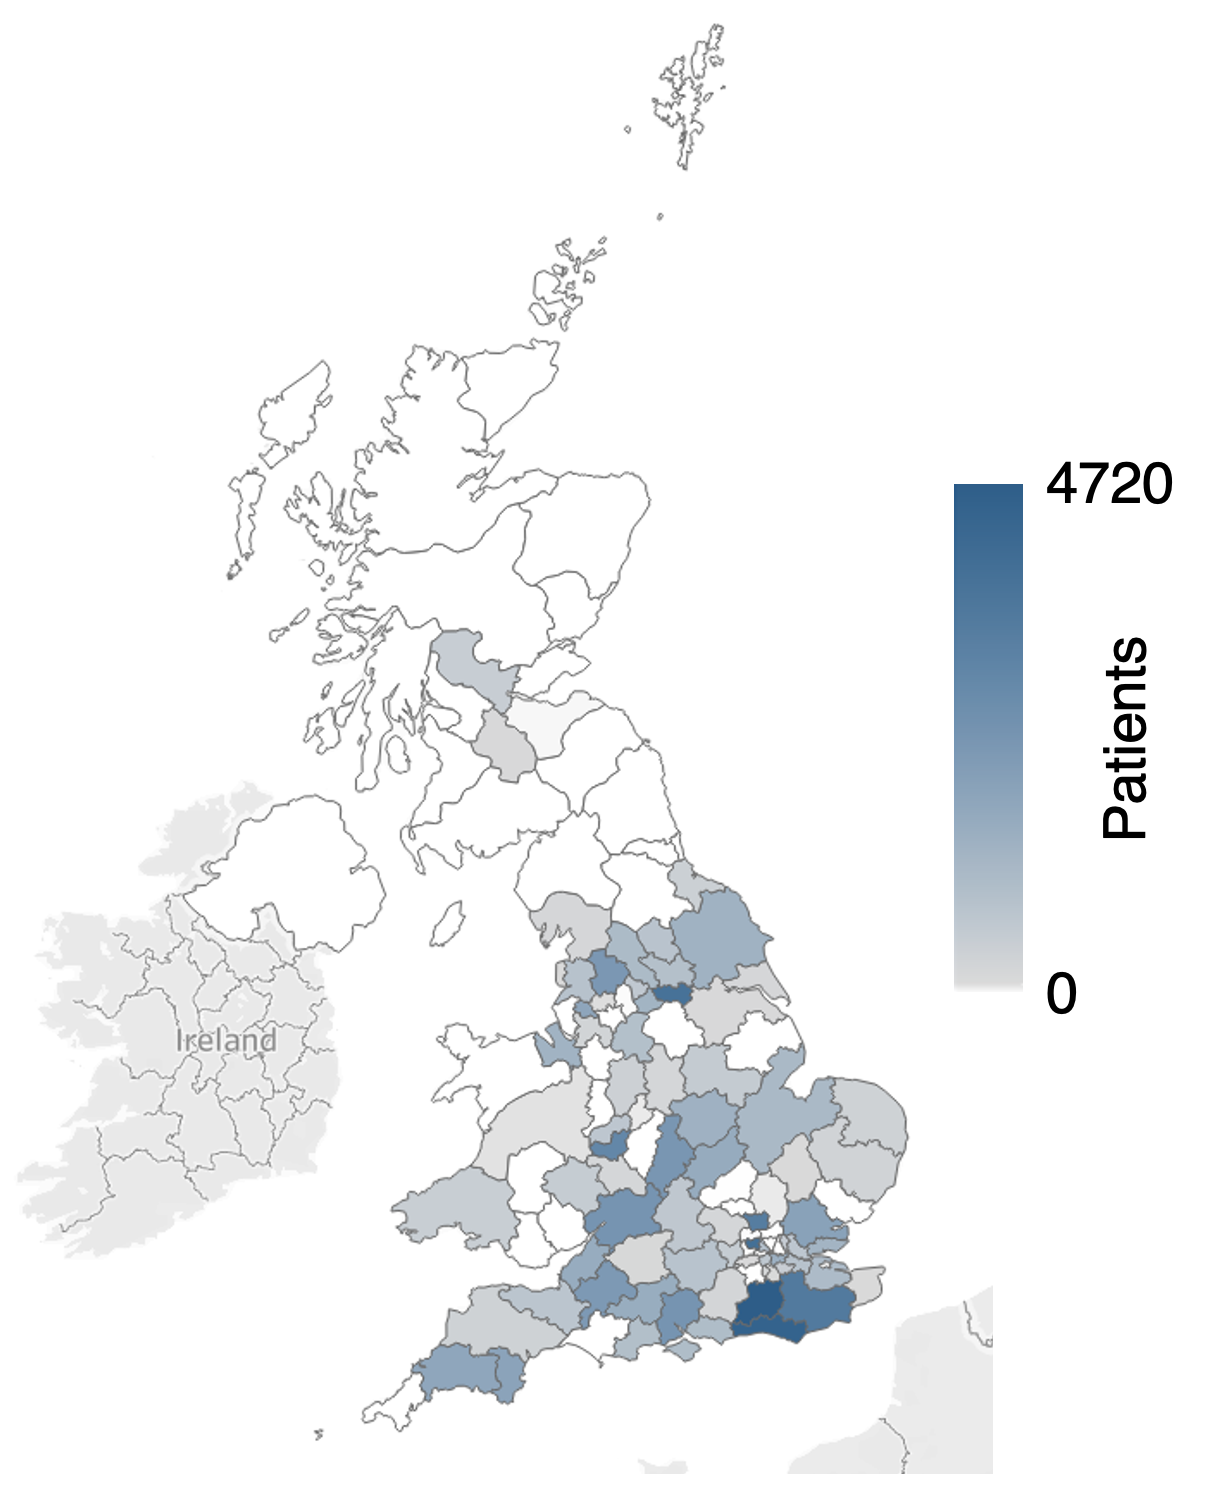
\includegraphics[width=0.5\textwidth]{uk_overview.png}
\caption{Distribution of processed patient locations within UK postal districts, for a subset of the complete datset.}
\label{uk_overview}
\end{figure}

Figure \ref{uk_overview} shows the geographic distribution of uploaded patient locations within the UK, for a subset of the complete dataset. Use of the service has been confined to England and Wales; by contrast Scotland and Northern Ireland have seen almost no use.  

\begin{figure}[H]
\centering
\includegraphics[width=\textwidth]{hists.png}
\caption{Histograms of user request characteristics. Left: total number of patients uploaded. Centre: request cluster size. Right: number of clusters per request.}
\label{hists}
\end{figure}

Figure \ref{hists} shows summary statistics of uploaded user requests. Users uploaded a median of 18 or mean of 33 patients per request with a target cluster size of around 10. Though a handful of users uploaded the maximum limit of 300 patients, a substantial minority uploaded 10 or so patients, resulting in a single cluster being generated. 

\subsection{Repeat detection}

Using a 21 day repeat threshold, 3,051 repeat requests were detected and removed from the dataset. The dataset was thus reduced from 9,501 requests covering 314,861 patients to 6,459 requests covering 198,023 patients. The latter figure represents the best estimate of the number of home visits that have been performed using the service. Of the repeats that remained within the dataset (separated by more than 21 days), some, but not all, could be consistent with second or booster vaccination doses. An example of a repeat that cannot be explained by vaccination is shown in figure \ref{a_repeat}: there are four occurrences across five months, all separated by at least one month. 

\begin{figure}[H]
\centering
\includegraphics[width=\textwidth]{a_repeat.png}
\caption{A single example of repeat usage that is inconsistent with vaccination: there are too many occurrences (four) over too short a time period (five months).}
\label{a_repeat}
\end{figure}


\subsection{Route planning}

Applied to the full dataset including repeats, the survey-derived lookup times and routing times of 37·0s and 4·7s per patient, respectively, yield an estimate of total time savings in planning of 3,647 hours, equivalent to 91 weeks at 40 hours/week. 


\subsection{Route following}

Applied to the full dataset without repeats, an empirical model of human performance on the TSP yields an estimate of the total savings in distance travelled of 37,368 km. This is equivalent to 747 hours, or 18 weeks at 40 hours/week, assuming a mean travel speed of 50 km/h or 30 mph. 

Combining the two time savings together yields a total of 4,394 hours of practitioner time, or 109 work-weeks. The time savings break down approximately in a 4:1 ratio for planning : travelling. Using mean salary estimates of £38k and £32k for a practice manager and community nurse respectively\footnote{Taken from \hyperlink{www.glassdoor.com}{www.glassdoor.com}}, these time savings can be converted into a cost saving of approximately £85k. 

\section{Discussion}

We have presented a simple and easy-to-use solution for optimising vaccine delivery to housebound patients. It has seen widespread use during the UK's Covid-19 vaccination campaign, reaching a substantial proportion of the target patient population, and yielded both time (over two years of practitioner time) and cost (approximately £85k) savings. One user in Plymouth reported doubling their rate of delivery using the service, a finding that implies \vm{} was able to reduce the burden on other parts of the healthcare system by quickly removing vulnerable patients from the unvaccinated population. 

Harder to quantify are the savings in cognitive load of automating the complicated process of route planning, but direct feedback from users (published on the \vm{} website) frequently touched on the `frustration' inherent to such a menial and labour-intensive task. This is especially relevant given the small number of users that uploaded requests containing the maximum allowed number of 300 patients; a manual approach for this number of patients would be infeasible. In light of the very low investment that was required to set up this service (the beta version was online in 48 hours), the overall cost-benefit ratio of this simple intervention is extremely favourable. 

The development of \vm{} relied upon real-time feedback from users. For example, the addition of walking directions (alongside driving) was made in response to requests from GP surgeries in urban areas. Given that neither the NHS nor any other central authority encouraged the uptake of this tool, it follows that widespread adoption was achieved entirely through word of mouth (in particular, GP networks on social media). This shows the importance of engaging directly with users before and during development to ensure their requirements are met, which is pertinent in light of the expectation that digital technologies will play an ever-greater role in primary care \cite{WorldHealthOrganizationWHO2018}. 

At the time of writing, the service is supporting the booster campaign. The underlying problem that the service addresses will however continue to exist long after Covid-19; namely, how to efficiently visit a set of patients subject to some constraint on group size? The underlying technology could therefore be applied in other domains. An obvious example, and one already suggested by multiple users, would be supporting annual flu vaccination campaigns; a more novel example would be supporting district nurses or community nurses in their day-to-day duties. Intriguingly, the analysis of repeat requests reveals use patterns that are inconsistent with vaccination, which in turn suggests that some users have already employed the service for other purposes. Given that community healthcare in the UK records around 100 million patient contacts annually with a budget of around £10 billion and one-fifth of the NHS workforce \cite{Fund2019}, the cumulative impact of efficiencies obtained at the grassroots level could be substantial. 

\section{Acknowledgements}

The authors acknowledge financial support provided by Magdalen College, Oxford, Oxford University Innovation, and JHubMed, part of UK Strategic Command. Support of a technical nature was provided by Microsoft Bing. 

\section{Supplementary material}

\subsection{Survey}

\paragraph{Cohort} There were 18 respondents, 6 female, with a mean age of 45 years ($\sigma$ = 20, minimum 26, maximum 78). Six respondents had occupations that are explicitly scientific, computing or data-focussed in nature. 

\paragraph{Questions} Three questions investigated lookup time. Respondents were presented with a list of postcodes of lengths 5, 8 and 13 respectively, and asked to locate them on map. They were allowed to use any tool to assist them in this, digital or otherwise, and were asked to record the time taken to complete each question. Three questions investigated routing time. Respondents were presented with scatter-plot distributions of points, sized 13, 20 and 26 respectively, and asked to generate routes with a target size of 7 to visit all locations in as short a distance as possible. Once again they were asked to record the time taken.

\paragraph{Analysis} In keeping with previous findings that human solution times scale linearly with problem size, linear regressions were performed on the survey responses to obtain estimates of lookup and planning time per patient. To each survey response, an extra datapoint of (0,0) was added to reflect the fact solution time should be negligible when there are no patients. Equivalently, this imposes the constraint that the $y$-intercept of the regressions should be close to zero. For both regressions, two extremely high survey response times were excluded as outliers, though they are presented in the results for completeness. 

\paragraph{Results} Figure \ref{lut_fit} shows the time taken to generate a spatial representation of a TSP as a function of the number of locations to be visited. A central estimate of 37·0s per location was derived from the regression ($R$ = 0·80). Figure \ref{planning_fit} shows the time taken to generate a set of routes from a spatial representation of a TSP as a function of the number of locations to be visited. A central estimate of 4·7s per location was derived from the regression ($R$ = 0·74). 

\begin{figure}[H]
\centering
\includegraphics[width=0.8\textwidth]{lut_fit.png}
\caption{Time taken to locate patients on a map, expressed as a midpoint in a 95\% confidence interval. Two survey responses were deemed outliers and excluded from the regression. The two extremely high response times came from respondents who used a physical map to complete the task (as opposed to a digital service such as Google Maps).}
\label{lut_fit}
\end{figure}

\begin{figure}[H]
\centering
\includegraphics[width=0.8\textwidth]{planning_fit.png}
\caption{Time taken to generate routes on a map, expressed as a midpoint in a 95\% confidence interval. Two survey responses were deemed outliers and excluded from the regression.}
\label{planning_fit}
\end{figure}

\subsection{Repeat analysis}

\begin{figure}[H]
\centering
\includegraphics[width=\textwidth]{many_repeats.png}
\caption{Selected examples of repeat requests separated by more than 21 days. Whilst some of these could be consistent with vaccination (ie, those with the longest interval), some repeats occur within around a month and so the explanation of these is uncertain.}
\label{many_repeats}
\end{figure}

Figure \ref{many_repeats} shows further examples of repeat requests with an interval of at least 21 days. Some repeats are sufficiently spaced apart to be consistent with vaccination and/or booster doses, though such an explanation is insufficient for those separated by a month or so. 


\bibliographystyle{unsrtnat}
\bibliography{../../../Documents/library.bib}

\end{document}